\documentclass[10pt,a4paper]{article}

\usepackage[a4paper,top=1.7cm,bottom=1.7cm,left=2.2cm,right=2.2cm,footskip=0.9cm]{geometry}
\usepackage{fontspec}
\usepackage{xeCJK}
\usepackage{amsmath}
\usepackage{graphicx}
\usepackage{booktabs}
\usepackage{tabularx}
\usepackage{array}
\usepackage[table]{xcolor}
\usepackage{titlesec}
\usepackage{enumitem}
\usepackage{caption}
\usepackage{float}
\usepackage[hidelinks]{hyperref}

% Fonts: PingFang TC for CJK, SF Pro for Latin
\setmainfont{SF Pro Text}[BoldFont={* Semibold}, ItalicFont={* Regular Italic}, BoldItalicFont={* Semibold Italic}]
\setsansfont{SF Pro Display}[BoldFont={* Semibold}]
% PingFang.ttc holds SC/TC/HK faces; select the TC ones by index
\setCJKmainfont{PingFang.ttc}[Path=/jupyter/fonts/中文/, FontIndex=2, BoldFont=PingFang.ttc, BoldFeatures={FontIndex=10}]
\setCJKsansfont{PingFang.ttc}[Path=/jupyter/fonts/中文/, FontIndex=2, BoldFont=PingFang.ttc, BoldFeatures={FontIndex=10}]
\xeCJKsetup{CJKecglue={\hskip 0.25em plus 0.08em minus 0.04em}}
% Typeset en dash, minus and arrows with the Latin font instead of as full-width CJK punctuation
\xeCJKDeclareCharClass{Default}{"2013, "2212, "2192, "00D7}

% Spacing: 10.5pt on 17.5pt leading for body text
\renewcommand{\normalsize}{\fontsize{10.5pt}{17.5pt}\selectfont}
\renewcommand{\small}{\fontsize{9.5pt}{15pt}\selectfont}
\renewcommand{\footnotesize}{\fontsize{8.5pt}{13pt}\selectfont}
\setlength{\parindent}{0pt}
\setlength{\parskip}{5pt}

\definecolor{accent}{HTML}{2A78D6}
\definecolor{ink}{HTML}{1D1D1F}
\definecolor{muted}{HTML}{6E6E73}
\definecolor{rule}{HTML}{D2D2D7}
\definecolor{todo}{HTML}{D03B3B}

\setlist{nosep,leftmargin=1.1em,topsep=3pt,itemsep=2pt}
\setlist[itemize]{label=\textcolor{accent}{\raisebox{0.1ex}{$\bullet$}}}
\usepackage{fancyhdr}
\usepackage{lastpage}
\fancyhf{}
\renewcommand{\headrulewidth}{0pt}
\cfoot{\footnotesize\color{muted}\thepage\ / \pageref*{LastPage}}
\pagestyle{fancy}

\titleformat{\section}{\sffamily\bfseries\fontsize{13pt}{18pt}\selectfont}{\textcolor{accent}{\thesection}}{0.6em}{}
\titlespacing*{\section}{0pt}{12pt}{4pt}

\captionsetup{font={footnotesize,color=muted},labelfont={bf,color=ink},labelsep=quad,skip=5pt}
\captionsetup[table]{name=表,position=top}
\captionsetup[figure]{name=圖}
\arrayrulecolor{rule}
\renewcommand{\arraystretch}{1.15}

% Values from the final notebook run; replace after it finishes.
\newcommand{\tbd}{\textcolor{todo}{待補}}
\newcommand{\nbssl}{91.33\%}
\newcommand{\kaggle}{90.00\%}

\newcommand{\keynum}[2]{%
  \begin{tabular}[t]{@{}c@{}}
    {\sffamily\bfseries\fontsize{17pt}{20pt}\selectfont #1}\\[1pt]
    {\footnotesize\color{muted}#2}
  \end{tabular}}

\begin{document}
\color{ink}

{\sffamily\bfseries\fontsize{18pt}{24pt}\selectfont DL Lab 3　半監督 Intel 場景影像分類}\hfill
{\color{muted}黃毓峰　315834011}

\vspace{6pt}
{\renewcommand{\arraystretch}{1}%
\begin{tabularx}{\linewidth}{@{}*{4}{>{\centering\arraybackslash}X}@{}}
\arrayrulecolor{ink}\toprule[0.8pt]\addlinespace[6pt]
\keynum{90.42\%}{Supervised val} &
\keynum{93.25\%}{Self-training val} &
\keynum{\nbssl}{Notebook 重跑 val} &
\keynum{\kaggle}{Kaggle public（notebook）} \\
\addlinespace[4pt]\arrayrulecolor{rule}\bottomrule
\end{tabularx}}

\section{方法}

\begin{minipage}[t]{0.49\linewidth}
\raggedright\setlength{\parskip}{5pt}
\textbf{模型}　自行實作的 Residual CNN，共 11.25M 參數，輸入 128×128。
Stem 是兩層 Conv 3×3 → BN → GELU。
主幹分 4 個 stage，寬度 64、128、256、512，各有 2 個 residual block。

Residual block 是 Conv 3×3 → BN → GELU → Conv 3×3 → BN → SE，加上 shortcut 後再過 GELU。
降採樣時 shortcut 改用 AvgPool 加 Conv 1×1。
正則化用 DropPath，機率從 0 線性增加到 0.2。

\textbf{Self-training}　先用 1800 張標註影像訓練 200 epoch。
之後每 \textit{N} 個 epoch 預測一次剩下的未標註影像，最大 softmax 機率 ≥ \textit{τ} 的就收下。
收下的標籤之後不再更動。
\end{minipage}\hfill
\begin{minipage}[t]{0.47\linewidth}
\vspace{-6pt}
\captionof{table}{最終超參數}
\small
\begin{tabularx}{\linewidth}{@{}>{\color{muted}}l >{\raggedright\arraybackslash}X@{}}
\toprule
Epochs & 200 + 200（supervised + self-training） \\
Optimizer & AdamW，batch 64 \\
Learning rate & 10\textsuperscript{−3} / 5×10\textsuperscript{−4}，cosine 到 10\textsuperscript{−5} \\
Warmup & 5 epoch，只用在 supervised \\
正則化 & Weight decay 0.05，label smoothing 0.1 \\
Pseudo-label & \textit{τ}~=~0.9，\textit{N}~=~5 \\
Augmentation & Crop 0.6–1、HFlip、TrivialAugment、Erasing \textit{p}~=~0.5 \\
\bottomrule
\end{tabularx}
\end{minipage}

\section{實驗設計}
每組實驗只改一個設定，以當下最佳為基準，seed 固定 2026，共 40 組。
指標是 self-training 後的最佳 val acc。
Val 有 1200 張，1 張等於 0.083\%，抽樣雜訊約 0.5\%（6 張）。

實驗用 notebook 的腳本版本執行，本文數字都來自腳本。
同一組設定在 notebook 重跑，結果比腳本低 0.7–1.9\%，最終設定為 91.33\%（腳本 93.25\%）。
差別只在亂數順序，所以 run 之間的變異約 2\%，比抽樣雜訊大。
單一改動的差距小於 2\% 時，只能當作趨勢。

\section{結果}
圖 \ref{fig:prog} 是採用的 6 項改動，val acc 從 89.58\% 提升到 93.25\%。
提升最多的是 RandomErasing \textit{p} 從 0.25 調到 0.5，增加 1.42\%。
加寬和 \textit{N}~=~5 各只多對 1–2 張，在雜訊範圍內。
每一步的 self-training 都比 supervised 高 1.1–2.8\%。

\begin{figure}[H]
\centering
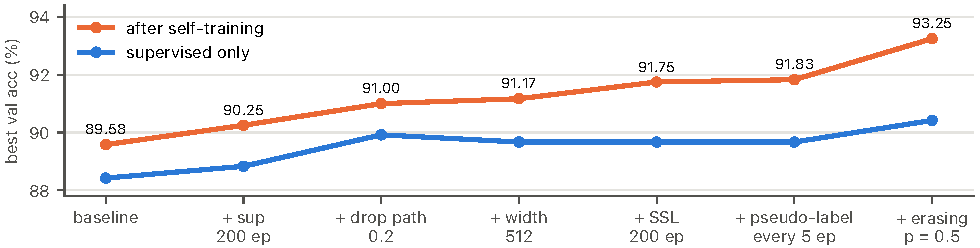
\includegraphics[width=\linewidth]{figures/progression.pdf}
\caption{逐步改動的最佳 val acc。每一步只在前一步上改一項。}
\label{fig:prog}
\end{figure}

\section{Activation function 比較}
以最終設定為基準，只替換 activation，SE block 裡的也一起換。
另外用早期設定（寬度 384、self-training 100 epoch、\textit{N}~=~10）再比一次。

\begin{table}[H]
\centering\small
\caption{三種 activation 的最佳 val acc（\%）}
\begin{tabular}{@{}l ccc c@{}}
\toprule
 & \multicolumn{3}{c}{最終設定} & 早期設定 \\
\cmidrule(lr){2-4}\cmidrule(l){5-5}
Activation & Supervised & Self-training & Pseudo-label 數 & Self-training \\
\midrule
GELU            & 90.42 & \textbf{93.25} & 3146 & \textbf{91.00} \\
ReLU            & 90.50 & 92.58 & 3171 & 90.25 \\
LeakyReLU (0.1) & 89.58 & 90.75 & 3153 & 90.75 \\
\bottomrule
\end{tabular}
\end{table}

\begin{figure}[H]
\centering
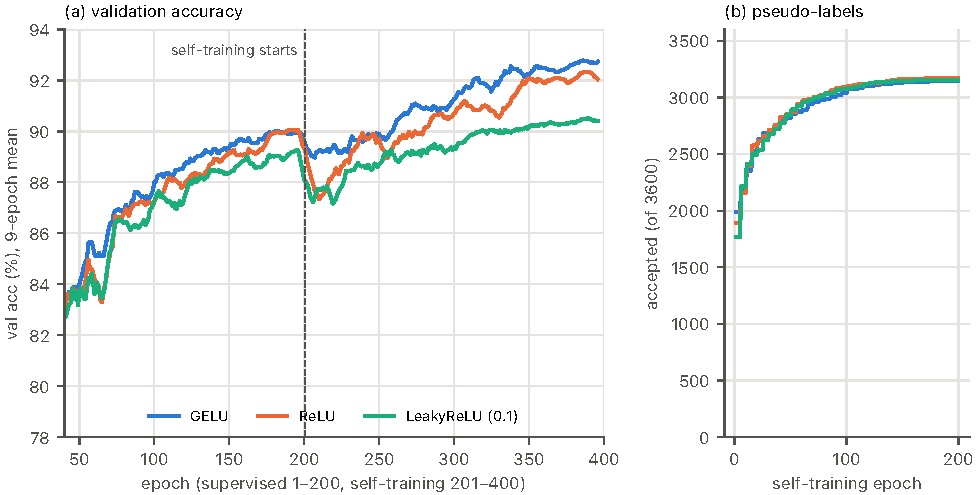
\includegraphics[width=\linewidth]{figures/activation.pdf}
\caption{(a) Val acc 的 9-epoch 移動平均。(b) 累計收下的 pseudo-label 數。}
\label{fig:act}
\end{figure}

\begin{itemize}
  \item \textbf{GELU 兩組都最好}。最終設定下比 ReLU 高 0.67\%，比 LeakyReLU 高 2.50\%。和 ReLU 的差距在 run 變異內，和 LeakyReLU 的差距較明確。
  \item \textbf{差距在 self-training 才拉開}。Supervised 階段三者差不到 1\%，見圖 \ref{fig:act}(a) 前 200 epoch。
  \item \textbf{Pseudo-label 數量相近}。三者都收了約 3150 張。推測差別在標籤正確率，錯誤會在後續輪次累積。未標註資料沒有真實標籤，這點無法直接驗證。
  \item \textbf{ReLU 和 LeakyReLU 的順序不穩定}。兩組設定的排序相反，差距在雜訊內。
  \item \textbf{原因無法確定}。LeakyReLU 在負值區也有梯度，卻沒有比 ReLU 好。所以「負值區有梯度」解釋不了 GELU 的優勢，平滑性可能也有影響。
\end{itemize}

\newpage
\section{消融實驗與錯誤分析}
表 \ref{tab:abl} 在最終設定上一次只改一項。
24 組全部低於基準，範圍 89.75–93.00\%。
同一設定在 notebook 重跑也只有 91.33\%，所以 93.25\% 很可能是 40 組裡偏高的一次。
多數差距在 run 變異內，下表只代表方向。

\begin{table}[H]
\centering\small
\caption{以最終設定（93.25\%）為基準的消融結果}
\label{tab:abl}
\begin{tabularx}{\linewidth}{@{}l r >{\raggedright\arraybackslash}X@{}}
\toprule
改動 & Δ val & 觀察 \\
\midrule
關閉 TrivialAugmentWide       & −3.50 & 影響最大的單一設定 \\
Label smoothing 0.1 → 0       & −2.33 & 收下 3570/3600 張，錯誤標籤一起進入訓練 \\
Batch size 64 → 128           & −1.92 & 更新步數減半，supervised 也下降 2.0 \\
Threshold 0.9 → 0.95          & −1.67 & 只收下 1299 張，資料不足 \\
Threshold 0.9 → 0.85          & −1.00 & 收下 3466 張，多收的多為雜訊 \\
Crop scale 下限 0.6 → 0.4     & −1.50 & 和 erasing 疊加後裁切過強 \\
RandomErasing \textit{p} 0.5 → 0.4   & −1.08 & 0.6、0.75 也都較差 \\
Depth (2,2,2,2) → (2,2,3,2)   & −1.08 & 參數增加 1.2M，沒有幫助 \\
輸入 128 → 144                & −1.00 & Supervised 上升 0.33，self-training 反而下降 \\
Self-training 200 → 300 epoch & −0.83 & 時間多 40\%，沒有提升 \\
\bottomrule
\end{tabularx}
\end{table}

\begin{itemize}
  \item \textbf{Augmentation 最關鍵}。只有 1800 張標註資料，關掉 TrivialAugment 的損失最大。
  \item \textbf{Val 的提升沒有完全反映到 test}。最初的 notebook 版本 val 90.25\%，Kaggle 89.60\%。最終設定在 notebook 是 91.33\% 與 90.00\%，在腳本是 93.25\% 與 90.20\%。Val 越高，和 Kaggle 的落差越大，表示用 val 挑選 40 組有過擬合。
  \item \textbf{Label smoothing 和 threshold 互相影響}。訓練目標的最高機率是 1 − \textit{ε} + \textit{ε}/\textit{K}~=~0.917。所以 \textit{τ}~=~0.95 幾乎收不到，\textit{τ}~=~0.9 剛好在上限之下。拿掉 label smoothing 後模型過度自信，threshold 就失去篩選作用。
\end{itemize}

\begin{minipage}[c]{0.44\linewidth}
\centering
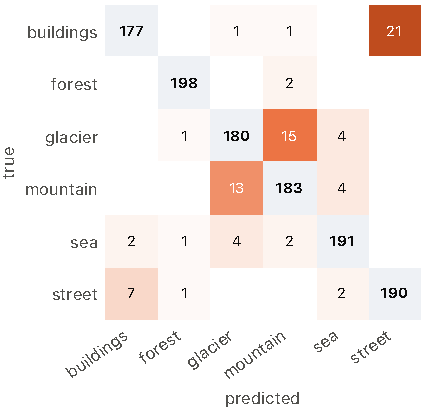
\includegraphics[width=\linewidth]{figures/confusion.pdf}
\captionof{figure}{最佳 checkpoint 的 val confusion matrix，顏色為錯誤率。}
\label{fig:cm}
\end{minipage}\hfill
\begin{minipage}[c]{0.52\linewidth}
\raggedright\setlength{\parskip}{5pt}
\textbf{錯誤集中在兩組相近類別}。
81 個錯誤裡有 56 個（69\%）來自這兩組。

Buildings 被判成 street 21 張，是最大的錯誤來源。
兩類都是城市街景，差別在主體是建築還是道路。

Glacier 和 mountain 互相誤判 28 張。
兩類都常同時出現雪和岩壁。

Forest 只錯 2 張，是最容易分的類別。
推測這些錯誤來自類別本身相近，這也和加深網路、放大輸入都沒有改善一致。
\end{minipage}

\vspace{8pt}
{\color{muted}\footnotesize 限制：每組只跑一次，無法估計標準差。Kaggle public：notebook 90.00\%，腳本 90.20\%，差距在變異內。}

\end{document}
